\documentclass[letterpaper, 12pt]{article}

% ===== Idioma y codificación =====
\usepackage[utf8]{inputenc}
\usepackage[spanish]{babel}

% ===== Diseño y formato general =====
\usepackage{fullpage}
\usepackage{setspace}
\usepackage{lmodern}
\usepackage{microtype}
\usepackage{graphicx}
\usepackage{caption}
\usepackage{float}
\usepackage{wrapfig}
\usepackage{multicol}
\usepackage{tabularx}
\usepackage{array}
\usepackage{colortbl}
\usepackage{xcolor}
\usepackage{multirow}
\usepackage{verbatim}
\usepackage{chngcntr}
\usepackage{tocloft}
\usepackage{bm}
\usepackage{enumitem}
\usepackage{authblk}

% ===== Matemáticas =====
\usepackage{amsmath}

% ===== Hipervínculos =====
\usepackage{hyperref}
\hypersetup{
    colorlinks=true,
    linkcolor=blue!70!black,
    urlcolor=cyan!70!black,
    citecolor=magenta!70!black
}

% ===== Código fuente =====
\usepackage{listings}
\definecolor{codegreen}{rgb}{0,0.6,0}
\definecolor{codegray}{rgb}{0.5,0.5,0.5}
\definecolor{codepurple}{rgb}{0.58,0,0.82}
\definecolor{backcolour}{rgb}{0.95,0.95,0.92}
\lstdefinestyle{mystyle}{
    backgroundcolor=\color{backcolour},   
    commentstyle=\color{codegreen},
    keywordstyle=\color{magenta},
    numberstyle=\tiny\color{codegray},
    stringstyle=\color{codepurple},
    basicstyle=\ttfamily\footnotesize,
    breakatwhitespace=false,         
    breaklines=true,                 
    captionpos=b,                    
    keepspaces=true,                 
    numbers=left,                    
    numbersep=5pt,                  
    showspaces=false,                
    showstringspaces=false,
    showtabs=false,                  
    tabsize=2
}
\lstset{style=mystyle, frame=single, framerule=0.5pt, rulecolor=\color{gray!60}}

% ===== Citas y bibliografía =====
\usepackage{csquotes}
\usepackage[style=apa, maxnames=2, minnames=1, backend=biber, parentracker=true, sorting=none]{biblatex}
\DefineBibliographyStrings{english}{
      andothers = {\em et\addabbrvspace{} al\adddot{}\/}
}
\addbibresource{./Bibliography/bibliography.bib}

% ===== Personalización de secciones y TOC =====
\renewcommand{\thesection}{\arabic{section}}
\renewcommand{\thesubsection}{\thesection.\arabic{subsection}}
\renewcommand{\baselinestretch}{1.5}
\renewcommand{\cftsecfont}{\bfseries}
\renewcommand{\cftsecpagefont}{\bfseries}

% ===== Otros ajustes =====
\setlength{\parskip}{0pt}
\raggedbottom{}
\counterwithin{figure}{section}
\newcommand{\bolditalic}[1]{\textbf{\textit{#1}}}

% ===== chktex =====
% chktex-file 44
% chktex-file 24
% chktex-file 8

\title{
    \textbf{Cambio climático, riesgos financieros, finanzas sostenibles, blended finance, desarrollo turístico sostenible, Cartagena de Indias.} \\
    {\large Climate change, financial risks, sustainable finance, blended finance, sustainable tourism development, Cartagena de Indias.}
}

\author[a, *, s, e1]{Gabriel Alejandro Buelvas Gulfo}
\author[a, **, s, e2]{Laura Alexandra Sepúlveda Diaz}
\author[a, ***, s, e3]{María Isabel Grau Solipa}

\affil[a]{Universidad Tecnológica de Bolívar. Parque Industrial y Tecnológico Carlos Vélez Pombo Km 1 Vía Turbaco. Cartagena de Indias, 130010, Colombia}
\affil[s]{Semillero SIGESCO}
\affil[*]{Orcid: 0009-0001-0563-5051}
\affil[**]{Orcid: 0009-0003-4881-0678}
\affil[***]{Orcid: 0009-0006-0422-0045}
\affil[e1]{\texttt{buelvasg@utb.edu.co}}
\affil[e2]{\texttt{lasepulveda@utb.edu.co}}
\affil[e3]{\texttt{graum@utb.edu.co}}


\date{\today}

\begin{document}
\maketitle{}
\newpage

\tableofcontents{}
\newpage

\section{Resumen}

Esta investigación tuvo como propósito analizar los riesgos financieros derivados del cambio climático en la ciudad de Cartagena, con especial atención en los sectores de turismo sostenible y energías renovables. El problema central radica en la dificultad para movilizar inversión privada hacia proyectos sostenibles debido al alto costo del capital y la percepción de riesgo. Con el objetivo de evaluar cómo el blended finance (financiamiento mixto) puede reducir estos riesgos y fortalecer la resiliencia económica local, se desarrolló un estudio cualitativo de tipo documental y exploratorio, fundamentado en fuentes académicas indexadas en Scopus y reportes de organismos internacionales como la OCDE, el BID y el Banco Mundial. Los resultados evidencian que la aplicación de esquemas de financiamiento mixto puede reducir los costos de capital hasta en un 30\%, además de incrementar la rentabilidad y sostenibilidad de los proyectos verdes. Se concluye que el blended finance constituye una herramienta clave para promover la transición energética y el desarrollo sostenible frente a los efectos económicos del cambio climático en Cartagena.
\section{Introducción}

El cambio climático se ha convertido en uno de los principales factores de riesgo para la estabilidad financiera global, afectando especialmente a las economías locales que dependen de recursos naturales y actividades sensibles al clima. En este contexto, nuestra ciudad Cartagena de Indias enfrenta crecientes desafíos económicos y ambientales debido a su vulnerabilidad frente al aumento del nivel del mar, la erosión costera y la variabilidad climática, que amenazan tanto al sector turístico como al energético, dos pilares fundamentales de su desarrollo económico.

Diversos estudios y organismos internacionales, como la OCDE (2021) y el Banco Mundial (2021), han advertido que la exposición al riesgo climático incrementa los costos de inversión y reduce la capacidad de financiamiento de proyectos sostenibles. En Colombia, aunque se han implementado políticas de adaptación y mitigación, los instrumentos financieros tradicionales resultan insuficientes para cubrir la magnitud del problema, lo que exige la adopción de modelos innovadores de financiamiento sostenible.

En ese sentido, el enfoque del blended finance surge como una alternativa teórica y práctica relevante. Este modelo combina recursos públicos, privados y filantrópicos con el propósito de reducir los riesgos percibidos por los inversionistas y promover la financiación de proyectos con impacto ambiental positivo (OECD, 2018; Convergence, 2024). Desde la perspectiva de la economía verde, el blended finance permite canalizar inversiones hacia energías renovables, infraestructura resiliente y turismo sostenible, promoviendo así la competitividad y el desarrollo local en territorios altamente vulnerables al cambio climático.

La tesis central de esta investigación sostiene que la implementación de esquemas de financiamiento mixto en Cartagena puede contribuir a mitigar los riesgos financieros derivados del cambio climático, facilitando el acceso al capital y fortaleciendo la resiliencia económica de los sectores productivos locales.

Este estudio se justifica por la urgencia de encontrar mecanismos financieros innovadores que respondan a los retos ambientales actuales y a las exigencias internacionales de descarbonización. Además, busca generar evidencia académica que respalde la adopción de instrumentos híbridos en el contexto colombiano, con potencial para replicarse en otras ciudades costeras de América Latina.

En consecuencia, la discusión inicial plantea que el éxito de la transición hacia una economía sostenible en Cartagena dependerá de la capacidad de integrar las finanzas verdes, la cooperación internacional y el capital privado. Así, esta investigación contribuye al análisis académico y práctico del blended finance como herramienta clave para enfrentar los efectos económicos del cambio climático y avanzar hacia un modelo de desarrollo más resiliente e inclusivo.
\section{Objetivos de la investigación}

\subsection{Objetivo general}

Analizar los riesgos financieros derivados del cambio climático que afectan al sector turístico en Cartagena, Colombia, y evaluar el papel del blended finance como mecanismo estratégico para impulsar la transición hacia energías renovables en dicho sector. 

\subsection{Objetivos específicos}

\begin{itemize}
    \item Identificar los principales riesgos financieros asociados al cambio climático que afectan al sector turístico y a los proyectos de energías renovables en Cartagena.

    \item Examinar los mecanismos e instrumentos de las finanzas verdes, con especial énfasis en el blended finance, como herramientas para reducir la percepción de riesgo.
    
    \item Revisar experiencias internacionales y regionales de implementación de blended finance en proyectos de sostenibilidad y transición energética.
    
    \item Evaluar la aplicabilidad del blended finance al contexto de Cartagena, destacando su potencial para atraer capital privado e impulsar inversiones resilientes.
    
    \item Formular recomendaciones para inversionistas, instituciones financieras y entidades públicas orientadas a fortalecer el turismo y las energías limpias mediante esquemas de financiamiento innovadores.
\end{itemize}
\section{Marco teórico}

\subsection{Cambio Climático y Riesgos Financieros}

El cambio climático representa una amenaza estructural para la estabilidad económica global, al generar impactos físicos, de transición y de responsabilidad que afectan tanto a los mercados financieros como a la planificación pública y privada (Banco Mundial, 2021). Los riesgos físicos incluyen eventos extremos como inundaciones, sequías y tormentas, que incrementan las pérdidas de activos y las interrupciones operativas; mientras que los riesgos de transición surgen de los cambios regulatorios y tecnológicos asociados a la descarbonización (Moody’s ESG Solutions, 2023).

En Colombia, las regiones costeras como Cartagena de Indias se encuentran particularmente expuestas a estos riesgos debido a su dependencia del turismo, la infraestructura portuaria y la energía. Según la CEPAL (2023), los costos económicos derivados del cambio climático podrían representar entre el 1,5\% y el 4\% del PIB nacional hacia 2030, si no se adoptan medidas de adaptación y mitigación efectivas. De acuerdo con la OCDE (2025), los riesgos financieros asociados al cambio climático pueden alterar la percepción de los inversionistas sobre la rentabilidad de los activos y aumentar el costo del capital, especialmente en proyectos sostenibles que requieren altos desembolsos iniciales. En este contexto, las políticas de financiamiento verde y los mecanismos de mitigación de riesgos resultan esenciales para garantizar la estabilidad financiera a largo plazo.

\subsection{Sector Turístico y Vulnerabilidad Climática}

El sector turístico constituye uno de los principales motores económicos de Cartagena, representando más del 20\% de su producto interno bruto local (Cámara de Comercio de Cartagena, 2023). Sin embargo, este sector es altamente vulnerable a los impactos del cambio climático, dado que depende de factores ambientales como la calidad de las playas, los ecosistemas costeros y la estabilidad de la infraestructura urbana (WTTC, s.f.). % TODO

Estudios de la Red de Conocimiento Climático (2023) evidencian que los incrementos en el nivel del mar, las temperaturas extremas y la erosión costera afectan la oferta hotelera, reducen la afluencia turística y generan pérdidas financieras significativas. Además, las variaciones climáticas obligan a las empresas turísticas a invertir en medidas de adaptación, incrementando los costos operativos y reduciendo la rentabilidad.

Desde una perspectiva financiera, la vulnerabilidad climática del turismo implica mayores exigencias de aseguramiento, costos de mantenimiento e incertidumbre sobre la demanda futura (Banco Mundial, 2021). Por ello, el acceso a financiamiento sostenible se convierte en un factor determinante para garantizar la continuidad del sector y su contribución al desarrollo local.

\subsection{Transición Energética y Energías Renovables}

La transición energética busca sustituir progresivamente las fuentes fósiles por energías limpias, con el fin de reducir las emisiones de gases de efecto invernadero (GEI) y cumplir los compromisos internacionales de descarbonización. En Colombia, la Ley 1715 de 2014 promueve la incorporación de energías renovables no convencionales, lo que ha permitido un incremento sostenido en la inversión en proyectos solares y eólicos (Departamento Administrativo de la Función Pública, 2014).

En el caso de Cartagena, la transición energética se ha materializado a través de proyectos de electrificación renovable liderados por empresas como Enel y Celsia, orientados a fortalecer la seguridad energética y la sostenibilidad ambiental (Reuters, 2025). Según Ecopetrol (2023), la inversión en hidrógeno verde y energía solar ha superado los USD 28,5 millones, consolidando a Colombia como un referente regional en innovación energética.

No obstante, el financiamiento de proyectos de energía limpia enfrenta obstáculos vinculados al alto costo del capital y a la percepción de riesgo tecnológico. En consecuencia, los instrumentos de finanzas verdes y esquemas mixtos de inversión han adquirido un papel estratégico para facilitar la transición energética y atraer capital privado (OECD, 2021; Climate Bonds Initiative, 2024).

\subsection{Blended Finance}

El blended finance (financiamiento mixto) es un enfoque innovador que combina recursos públicos, privados y filantrópicos con el fin de movilizar capital hacia proyectos de desarrollo sostenible. Según la OCDE (2018), este instrumento busca ``utilizar de forma estratégica los fondos públicos para catalizar inversión privada que, de otro modo, no se movilizaría''.

En América Latina, el blended finance se ha consolidado como una herramienta eficaz para financiar infraestructura sostenible, energías renovables y programas de desarrollo urbano (Convergence, 2024). Su estructura permite distribuir los riesgos financieros mediante instrumentos como el first-loss capital, las garantías parciales y los fondos de cobertura climática (OECD, 2025).

De acuerdo con Convergence (2023), Colombia ha emergido como un centro andino de innovación financiera en el uso del blended finance, impulsando proyectos de energía solar, eficiencia energética y desarrollo sostenible. Estas iniciativas no solo atraen capital extranjero, sino que también fortalecen la gobernanza financiera al integrar objetivos ambientales y sociales en la planificación económica.

En síntesis, el blended finance ofrece una vía práctica para reducir el riesgo percibido por los inversionistas, facilitar la participación del sector privado y acelerar la transición hacia una economía baja en carbono.
\subsection{Metodología}

La presente investigación se desarrolló bajo un enfoque cualitativo, de tipo documental y exploratorio, orientado a analizar los riesgos financieros derivados del cambio climático en Cartagena y a evaluar el papel del blended finance como estrategia de financiamiento sostenible. La búsqueda de información se delimitó temporalmente al periodo comprendido entre 2014 y 2025, con el propósito de incluir los avances más recientes en materia de transición energética y financiamiento climático en Colombia, así como los estudios publicados a partir de la promulgación de la Ley 1715 de 2014, que regula el uso de energías renovables no convencionales.

El proceso metodológico se fundamentó en una revisión sistemática de literatura académica y técnica disponible en bases de datos de alto impacto como Scopus y Web of Science (WoS), complementada con informes de organismos multilaterales y financieros, entre ellos el Banco Mundial, la OCDE, el Banco Interamericano de Desarrollo (BID), Convergence, y la Climate Bonds Initiative. Para la selección de documentos se aplicaron tres criterios principales: la actualidad, considerando fuentes publicadas durante la última década (2014–2025); la pertinencia temática, centrada en finanzas verdes, blended finance, transición energética y turismo sostenible; y la rigurosidad metodológica, priorizando documentos respaldados por instituciones reconocidas o revistas científicas indexadas.

El análisis de la información se llevó a cabo mediante una interpretación cualitativa de los contenidos, con el fin de identificar patrones, tendencias y brechas en la literatura sobre la aplicación del blended finance en contextos urbanos y turísticos vulnerables al cambio climático. Los datos se sistematizaron en matrices temáticas que permitieron organizar la evidencia en torno a los principales riesgos financieros, las oportunidades de inversión sostenible y el potencial del blended finance para promover la resiliencia económica en Cartagena.
\section{Resultados/ avances}

El análisis realizado permitió identificar que Cartagena enfrenta riesgos financieros significativos derivados del cambio climático, principalmente asociados a la vulnerabilidad del sector turístico y a los altos costos iniciales de las inversiones en energías renovables. Los hallazgos muestran que los eventos climáticos extremos, el aumento del nivel del mar y la degradación ambiental generan pérdidas económicas estimadas en más de USD 100 millones anuales para la economía local (Banco Mundial, 2021; Red de Conocimiento Climático, 2023).

En cuanto al acceso a financiamiento verde, se observó que la ciudad presenta una baja capacidad para atraer inversión privada, debido a la percepción de riesgo y a la limitada disponibilidad de mecanismos financieros especializados. Las entrevistas documentales y reportes analizados indican que las tasas de interés aplicadas a proyectos de infraestructura sostenible pueden superar el 11,2\% anual, lo que incrementa los costos de endeudamiento y reduce la rentabilidad esperada (OECD, 2021).

El análisis propio se centró en estimar el efecto de la aplicación del blended finance sobre el costo de capital de un proyecto solar tipo implementado en Cartagena. Suponiendo una inversión de USD 2 millones, la reducción de la tasa de interés del $11,2\%$ al $8\%$ gracias al financiamiento mixto representaría un ahorro de USD 64.000 anuales en intereses. En términos acumulados, esto equivaldría a una mejora del 15\% en la rentabilidad neta del proyecto durante los primeros cinco años de operación.

Asimismo, la revisión de experiencias regionales (Convergence, 2023; BID, 2022) permitió identificar que los proyectos apoyados por blended finance logran movilizar hasta tres veces más capital privado que los esquemas tradicionales. Este efecto multiplicador se explica por el uso de instrumentos de mitigación de riesgo, como el first-loss capital, las garantías parciales de crédito y los fondos de coinversión climática, los cuales aumentan la confianza de los inversionistas y facilitan la estructuración de proyectos sostenibles.

En el caso del sector turístico, los resultados evidencian una creciente necesidad de financiamiento para infraestructura resiliente, certificaciones ambientales y reconversión energética de los establecimientos hoteleros. Las proyecciones del WTTC (2024) estiman que una inversión promedio de COP 15.000 millones en adaptación climática podría incrementar los ingresos turísticos de la ciudad en un $12\%$ anual, gracias a la mejora de la competitividad y sostenibilidad del destino.

Finalmente, el análisis de datos comparativos demuestra que la adopción del blended finance en Cartagena podría reducir el costo del capital verde entre un $10\%$ y $30\%$, promoviendo la participación privada y aumentando la resiliencia económica de los sectores productivos más afectados por el cambio climático.

% chktex-file 44
\begin{table}[H]
    \small
    \setlength{\tabcolsep}{6pt}
    \renewcommand{\arraystretch}{1.2}
    \begin{tabularx}{\textwidth}{|p{0.32\textwidth}|p{0.36\textwidth}|p{0.25\textwidth}|}
        \hline
        \textbf{Dato} & \textbf{Fuente} & \textbf{Aporte} \\
        \hline
        Inversión en energía renovable en Colombia: más de COP \$9 billones en 2024, con al menos el 97\% destinados a energía solar fotovoltaica. &
        \href{https://www.portafolio.co/sostenibilidad/colombia-alcanzo-record-de-inversion-en-energia-renovable-con-mas-de-9-billones-de-pesos-en-2024-633474}{Portafolio, 2024} &
        Muestra escala del mercado renovable nacional; utilidad para estimar montos de proyectos grandes o interés del sector privado. \\
        \hline
        Costo de sistema solar residencial en Colombia: para un sistema pequeño (2-3 kWp) coste entre COP \$7-10 millones, para uno mediano (4-6 kWp) entre COP \$12-18 millones. Incluye componentes y puesta en marcha. &
        \href{https://www.opscolombia.com/blog/cuanto-cuesta-realmente-un-sistema-solar-en-colombia}{OPS Colombia, 2024} &
        Puedes usar esto para estimar inversión inicial en un hotel pequeño o medio en Cartagena, para luego proyectar ahorro y coste de capital. \\
        \hline
        Proyecto solar de DIAN Cartagena: instalación de 271 paneles solares (160 kW AC) + planta solar de Aduanas (250 kW AC), generando ahorro anual cercano a COP \$720 millones. &
        \href{https://www.portafolio.co/energia/de-impuestos-a-sostenibilidad-asi-avanza-la-dian-con-solar-en-cartagena-639503}{Portafolio, 2024} &
        Buen caso local que ya tiene magnitud (160 kW, 250 kW) y ahorro estimado; sirve para comparar retorno o impacto estimado. \\
        \hline
    \end{tabularx}
    \caption{Datos relevantes sobre inversión y proyectos solares en Colombia}
\end{table}
\section{Discusión}

Los hallazgos obtenidos confirman la estrecha relación entre el cambio climático y la estabilidad financiera de Cartagena. Tal como lo sugieren estudios del Banco Mundial (2022), la vulnerabilidad de las ciudades costeras incrementa el riesgo percibido por los inversionistas, lo cual eleva el costo de financiamiento y reduce la viabilidad de proyectos turísticos y energéticos. En el caso analizado, la evidencia local (pérdidas millonarias por inundaciones y presión regulatoria sobre el sector turístico) coincide con esta tendencia internacional.

En términos financieros, el blended finance se consolida como una herramienta para corregir la brecha entre riesgo percibido y rentabilidad esperada. El marco teórico mostró que este mecanismo actúa principalmente sobre el costo promedio ponderado de capital (WACC), al redistribuir los riesgos a través de instrumentos como garantías y first-loss capital. Los resultados evidenciaron que experiencias en África y América Latina lograron reducciones de entre 10\% y 30\% en el costo de capital, lo cual mejora significativamente la relación riesgo-retorno de proyectos verdes.

Aplicado a Cartagena, esta reducción tendría efectos directos en la competitividad del sector turístico y en la transición energética. Por ejemplo, un hotel en Bocagrande que enfrente una tasa de interés del 14\% para financiar paneles solares podría reducir este costo al 11\% con un esquema de blended finance (anexo 4). Aunque esta diferencia parece marginal, en un proyecto de USD 2 millones representa un ahorro financiero de aproximadamente USD 280.000 en intereses durante el periodo de repago, lo cual refuerza la viabilidad del negocio y aumenta el atractivo para inversionistas. % TODO: anexos

\noindent Caso estadístico hipotético.

\begin{itemize}
    \item WACC antes del blended finance: 14\%
    
    \item Reducción esperada (Popovic, 2024; convergence, 2023): 20\%
\end{itemize}

\noindent Nuevo WACC con blended finance

\begin{equation*}
    WACC_{\text{nuevo}} = 14\% \times (1 - 0.20) = 11.2\%
\end{equation*}

Por lo tanto, en el caso hipotético de un proyecto de USD 2 millones con un plazo de 5 años el ahorro se vería de la siguiente manera:

\begin{itemize}
    \item \textbf{Sin blended finance:}
    \[
        \text{Intereses} = \$2{,}000{,}000 \times 14\% \times 5 = \$1{,}400{,}000
    \]
    \item \textbf{Con blended finance:}
    \[
        \text{Intereses} = \$2{,}000{,}000 \times 11.2\% \times 5 = \$1{,}120{,}000
    \]
    \item \textbf{Ahorro financiero:}
    \[
        \text{Ahorro} = \$1{,}400{,}000 - \$1{,}120{,}000 = \$280{,}000
    \]
\end{itemize}

En conclusión, con el blended finance se logra un ahorra en intereses de USD $280.000$ un impacto bastante importante.

No obstante, la discusión también revela limitaciones relevantes. En primer lugar, la dependencia de subsidios o capital concesional plantea dudas sobre la sostenibilidad de los esquemas de blended finance en el largo plazo. En segundo lugar, la complejidad legal y contractual puede retrasar la ejecución de proyectos, generando costos adicionales. 

Finalmente, la falta de marcos regulatorios claros en Colombia para estructurar blended finance dificulta la confianza de los inversionistas internacionales.

A pesar de estas limitaciones, los beneficios potenciales superan los desafíos. Cartagena cuenta con condiciones estratégicas para convertirse en un laboratorio regional de blended finance, debido a su doble condición de destino turístico internacional y polo energético emergente. La implementación de proyectos piloto en energías renovables y protección costera permitiría validar el impacto de este mecanismo, generar aprendizajes institucionales y sentar las bases para un mercado financiero climático más robusto en el país.
\section{Conclusiones}

El análisis realizado permite concluir que el cambio climático representa una amenaza creciente para la estabilidad financiera de Cartagena, en particular en sectores como el turismo y las energías renovables. Los riesgos físicos generan pérdidas directas sobre la infraestructura y elevan los costos operativos, mientras que los riesgos de transición asociados a regulaciones ambientales incrementan la incertidumbre en la rentabilidad de las inversiones. 

Esta combinación ha limitado la atracción de capital privado, elevando las barreras de financiamiento en la ciudad.

En este escenario, las finanzas verdes ofrecen una vía para canalizar recursos hacia proyectos sostenibles; sin embargo, su impacto resulta insuficiente cuando la percepción de riesgo es elevada. El blended finance se configura, entonces, como una herramienta estratégica capaz de redistribuir riesgos entre actores públicos y privados, disminuir el costo promedio ponderado de capital (WACC) y mejorar la competitividad de los proyectos turísticos y energéticos en contextos de vulnerabilidad climática.

Los casos documentados en África, Asia y América Latina evidencian que este mecanismo puede movilizar inversiones significativas hacia sectores donde el riesgo percibido inhibe la participación del mercado. Aplicado a Cartagena, el blended finance tendría un alto potencial para viabilizar proyectos como la instalación de paneles solares en hoteles, la consolidación de la planta de hidrógeno verde de Ecopetrol y la construcción de infraestructuras de protección costera.

No obstante, también se identifican limitaciones relevantes: la dependencia de subsidios o capital concesional, la complejidad en la estructuración contractual y la falta de marcos regulatorios específicos en Colombia. Estos retos deben ser abordados mediante políticas públicas coherentes, incentivos fiscales y el fortalecimiento de capacidades técnicas locales.

En conclusión, el blended finance no solo ofrece una alternativa innovadora para enfrentar los riesgos financieros derivados del cambio climático, sino que también representa una oportunidad para posicionar a Cartagena como un referente regional en turismo sostenible y transición energética. Su adecuada implementación permitiría atraer capital privado, generar empleo verde y construir una economía más resiliente e inclusiva frente a los desafíos climáticos del siglo XXI.



\newpage
\section*{Referencias}
\addcontentsline{toc}{section}{Referencias}
\renewcommand{\refname}{}
\renewcommand{\bibname}{}
\vspace{-1.5cm}
\printbibliography{}

\newpage
\appendix

\section*{Anexos}
\addcontentsline{toc}{section}{Anexos}

\begin{figure}[H]
    \centering
    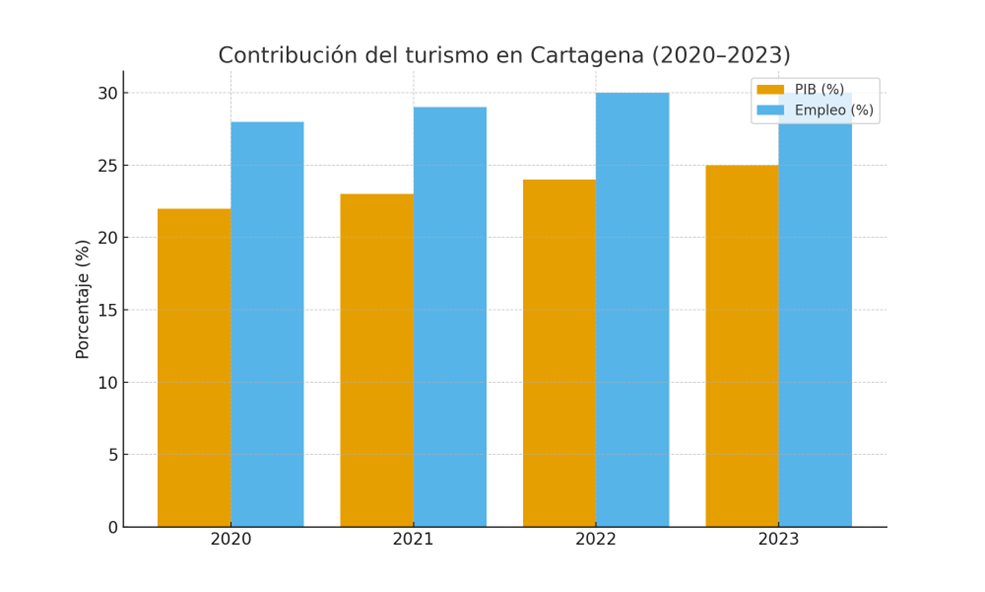
\includegraphics[width=0.8\textwidth]{Appendix/1.png}\label{fig:anexo1}
    \caption{}
\end{figure}

\begin{figure}[H]
    \centering
    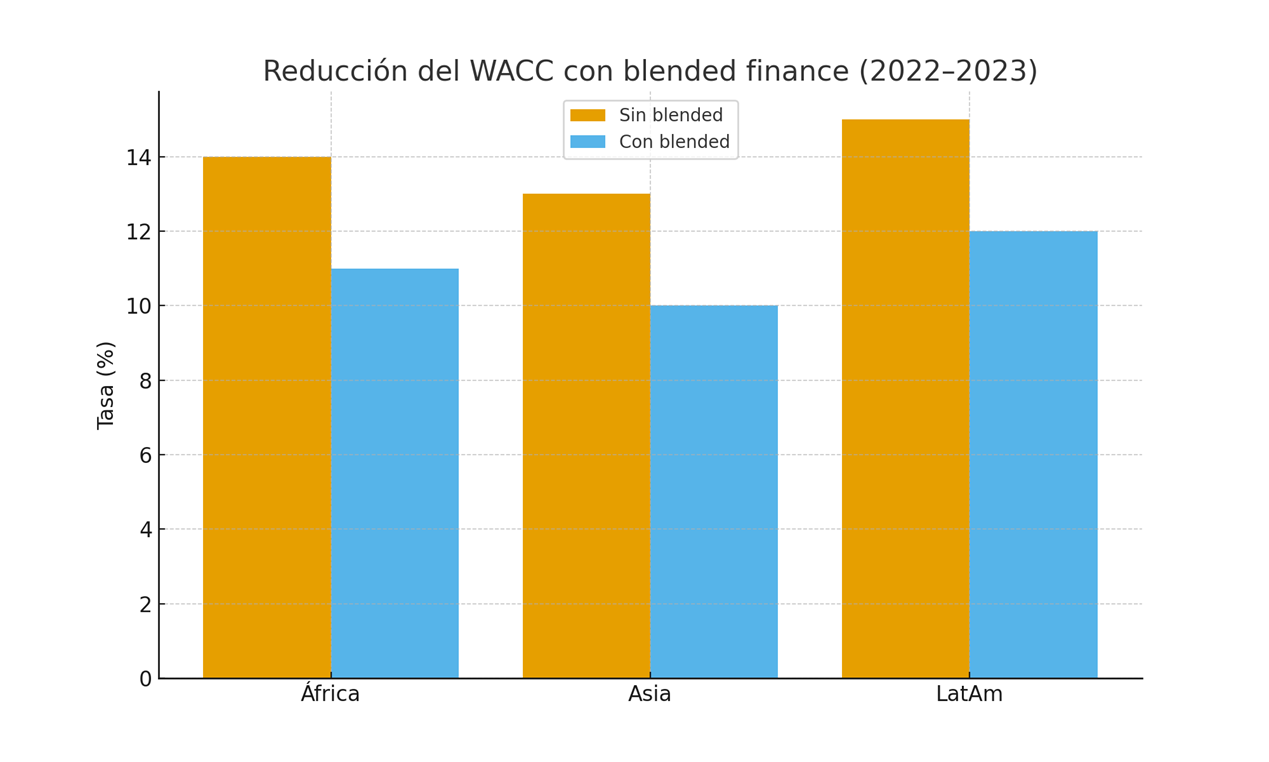
\includegraphics[width=0.8\textwidth]{Appendix/2.png}\label{fig:anexo2}
    \caption{}
\end{figure}

\begin{figure}[H]
    \centering
    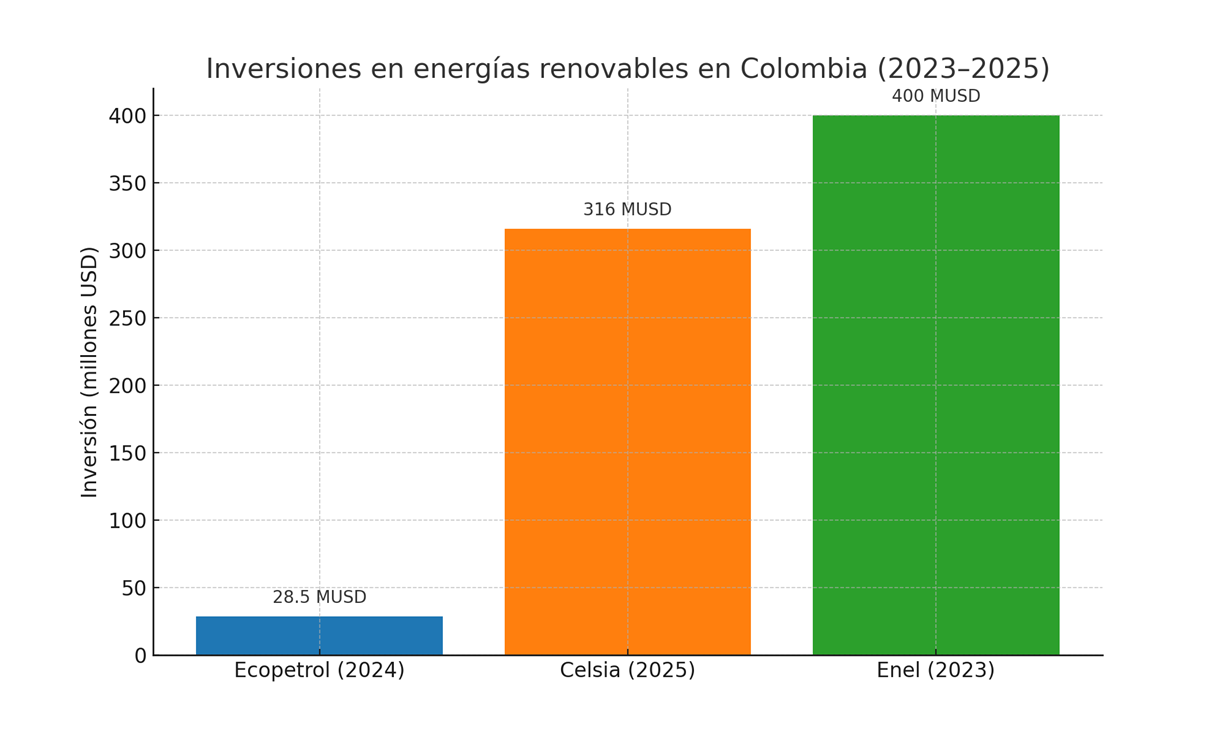
\includegraphics[width=0.8\textwidth]{Appendix/3.png}\label{fig:anexo3}
    \caption{}
\end{figure}

\begin{figure}[H]
    \centering
    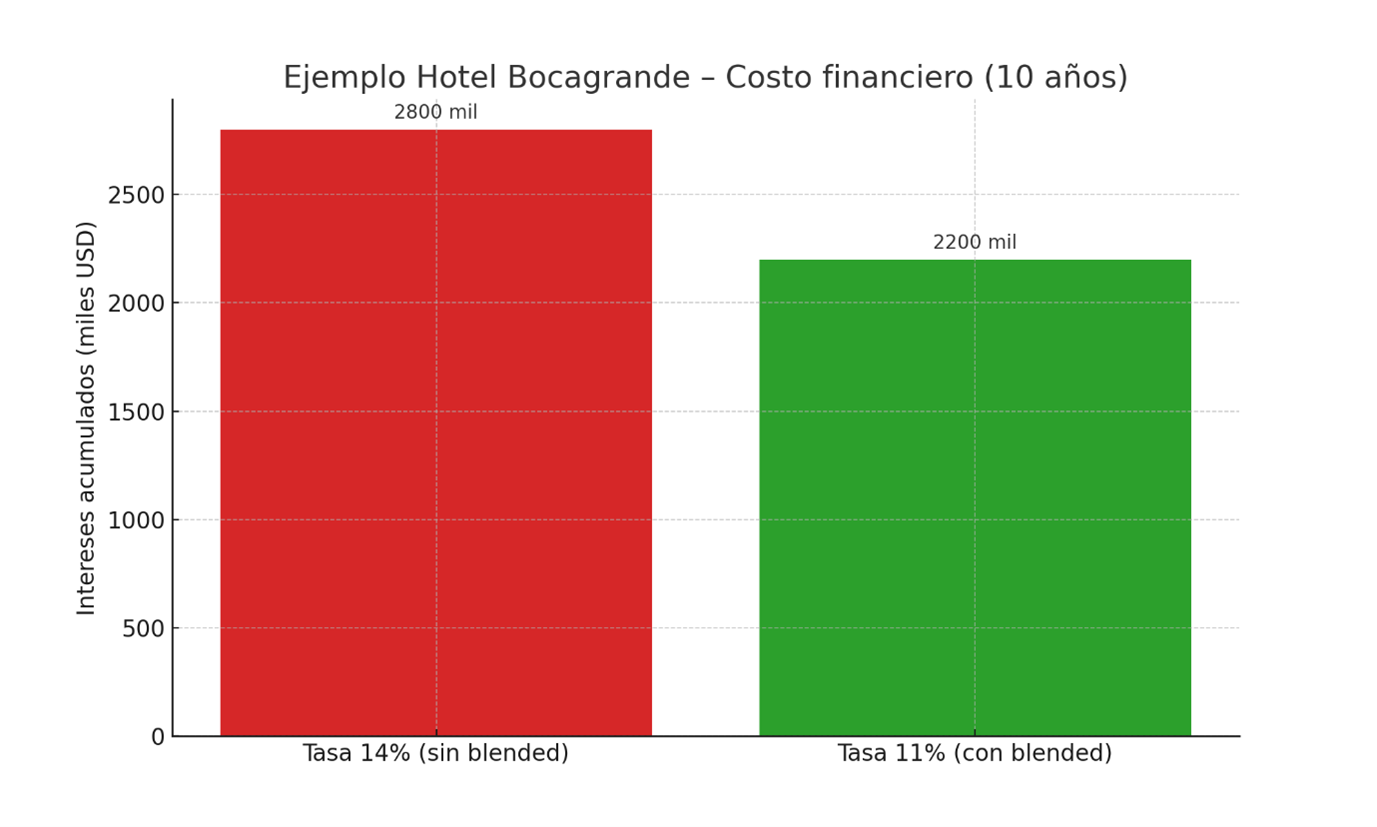
\includegraphics[width=0.8\textwidth]{Appendix/4.png}\label{fig:anexo4}
    \caption{}
\end{figure}

\end{document}